\subsubsection{Neuro-Symbolic Integration approaches} \label{nsi_approaches}
The first boundary between NSI approaches can be drawn with respect to the field for which they are designed. We can identify two main areas where these approaches are applied: machine learning and symbolic reasoning. In the first case, the integration aims to regulate the learning process with the use of logical knowledge. The goal of this family of approaches is to exploit the computational efficiency of DNNs and the expressiveness of logic to improve neural model capabilities in classical machine learning tasks, ranging from classification (e.g., binary, multiclass, multilabel, collective) to embedding learning, also covering relational learning tasks. On the other hand, we can find NSI approaches that are designed to solve problems from the symbolic field. In this second family of approaches, a DNN is trained to learn and perform symbolic reasoning over knowledge. The target of these works is more about Inductive Logic Programming (ILP) tasks and related.

Another possible distinction between NSI works concerns the adopted logical language. Looking at the approaches proposed in the literature, we can notice that there is not a standard way to represent logical knowledge. In most cases, a set of FOL rules is used to set constraints on data. However, a lot of approaches relying on this kind of rules apply some restrictions to the language, thus limiting its expressiveness. Such restrictions may involve the arity of predicates, functions, and logical operators. Other limitations may be imposed on the form that must be used to express logical rules (e.g., Horn clauses). Furthermore, additional assumptions can involve the usage of variable quantifiers (e.g., universal assumption). Most of these restrictions do not affect the approaches based on propositional logic. However, propositional logic is less expressive and flexible than FOL by definition.

Even the semantics of the logical language can differ a lot from one approach to another. If the goal is to have an end-to-end fully differentiable architecture, then it will be necessary to move away from finite-valued logic. The motivation behind this need derives from the nature of neural networks, which deal with continuous real values. For this reason, the most frequent solution is to relax the logic by adopting fuzzy/probabilistic semantics. In this way, it is possible to evaluate logical formulas grounded with values coming from a neural network. The main benefit that derives from the use of infinite-valued logic is that it allows to efficiently train a Neuro-Symbolic model using back-propagation algorithms. As discussed in section \ref{fuzzy_logic}, there are many possible choices between fuzzy operators. Each of them behaves in different ways when used in a differentiable learning setting. In~\cite{analyzingDiffFuzzyLogic} several experiments were performed to show the weakness and strengths of different fuzzy operators.

After this NSI overview about logical language and semantics, we can go deeper and categorize the state-of-the-art works. As proposed in~\cite{ltn}, a reasonable way to group the novel approaches is to consider the methodology adopted to inject logical knowledge into the learning process. In Figure~\ref{fig:sota} we can see three main groups. Each of them is based on different architectures.
\begin{figure}
    \centerline{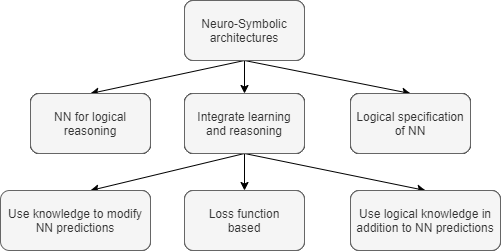
\includegraphics[scale=.58]{sota.png}}
    \caption{Categorization proposed in~\cite{ltn} to group Neuro-Symbolic approaches based on the knowledge injection methodology}
    \label{fig:sota}
\end{figure}
\\\\
\textit{\textbf{Neural architectures for logical reasoning:}}~\cite{tensorlog,cohen2020scalable,conditionalTheoremProvers,campero2018logical,neuralMarkovLogicNetworks,probabilisticLogicNeuralNetworks,recursiveReasoningNetworks,deepProlog,satnet,nlrl}. These approaches use neural networks to perform probabilistic inference on logical theories by learning reasoning strategies. This category focuses mainly on ILP (e.g., theory learning, theory compression, logical rule induction) and structured data-related tasks (e.g., knowledge graph completion, knowledge graph reasoning, triple classification). The proposed methodologies reach their goals in various ways.

Starting from~\cite{probabilisticLogicNeuralNetworks}, we find Probabilistic Logic Neural Networks. The proposed models are defined to perform knowledge graph reasoning. A Markov Logic Network~\cite{markovLogicNetworks} is used to compute the joint distribution of all triplets, then a model is trained with a variational expectation-maximization algorithm. Another approach based on Markov Logic Networks is~\cite{neuralMarkovLogicNetworks}, in which a statistical relational learning system is proposed to learn the implicit representation of FOL rules through neural networks.

Going on, we find~\cite{recursiveReasoningNetworks},~\cite{campero2018logical} and~\cite{tensorlog}. All of them introduce some FOL language restrictions, supporting only unary and binary predicates. In~\cite{recursiveReasoningNetworks}, Hohenecker and Łukasiewicz introduce Recursive Reasoning Networks. In this approach, each training example is a KB composed of different facts. Models are trained on these KBs using a shared ontology, then generate embeddings of individuals. Moving on to~\cite{campero2018logical}, Campero et al. propose a task-dependent loss function. Their methodology relies on forward chaining and soft unification to perform inference. Then there is TensorLog~\cite{tensorlog}, where a subset of FOL called \textit{ptree-SDKGs} is provided to represent knowledge in a highly scalable framework for tuning parameters of probabilistic logic. 

To conclude with the last three approaches of this family, we find the methodology proposed by Cohen et al.~\cite{cohen2020scalable}, Conditional Theorem Provers (CPT)~\cite{conditionalTheoremProvers}, and SATNet~\cite{satnet}. Cohen et al. propose \textit{sparse-matrix reified KBs} to represent subjects, objects, and relations of a KB. Through these three sparse matrices, they provide an effective and scalable way to represent symbolical knowledge in neural contexts. Moving on to CPT, Minervini et al. propose a method to boost the efficiency of a model in a particular way: during the proving mechanism, the learning process aims to dynamically select only a minimal subset of rules depending on the current goal. At last, we have SATNet by Wang et al.. In this approach, a MaxSAT solver layer is used to make DNNs able to learn logical structures without explicitly specifying any logical rules. Both CPT and SATNet adopt a logical language that is function-free.
\\\\
\textit{\textbf{Logical specification of neural network architectures:}}~\cite{liftedRelationaNeuralNetworks,logicalNeuralNetworks}. In these novel approaches, a logical language is used to specify the architecture of neural networks. This peculiarity leads to better interpretability of DNNs.

In~\cite{liftedRelationaNeuralNetworks}, Sourek et al. propose Lifted Relational Neural Networks. These neural models are composed of multiple feed-forward networks (one per example) with shared weights, where each node represents a weighted clause. The methodology proposed in Logical Neural Networks~\cite{logicalNeuralNetworks} is quite different. In this case, a neural network is modeled as a graph representing the syntax tree of logical formulas. The knowledge is expressed through a function-free FOL language with \textit{weighted nonlinear logic} semantics.

In both approaches, clause weights are learnable parameters. This feature makes the model able to give greater importance to the more relevant rules at prediction time.
\\\\
\textit{\textbf{Neuro-symbolic architectures for the integration of inductive learning and deductive reasoning:}} The goal of this group of approaches is to integrate neural and logical components into a unique (possibly fully differentiable) framework. In this way, the processes of learning and reasoning of the two components influence each other to enhance the quality of predictions. Unlike the previous categories, these works are more oriented to exploit logical knowledge in classical machine learning tasks. This family of architectures can be further divided into three subclasses:
\begin{itemize}
    \item \textbf{\textit{Logical knowledge to modify neural networks predictions:}}~\cite{liSrikumar,rnm,dlm,kenn}. These works rely on additional components (e.g., neurons, layers, modules) responsible for handling the logical knowledge.
    
    Li and Srikumar~\cite{liSrikumar} propose a framework to introduce constraints as logical statements without adding any extra learnable parameters. The base neural model is augmented with \textit{named neurons} corresponding to the predicates of the logical clauses. The post-activation value of a named neuron can be seen as the truth value of the mapped predicate. About the language, rules must be expressed as logical implications with some restrictions: the antecedent is a conjunction/disjunction of literals and the consequent is a single literal. 
    
    The second approach of this family is the one proposed by Daniele and Serafini with Knowledge Enhanced Neural Networks (KENN)~\cite{kenn}. The logical knowledge is injected through an additional layer called \textit{Knowledge Enhancer}. The initial predictions of the base neural network are modified through this layer to increase the satisfaction of each clause by applying a boost function. The logical language is a restricted function-free FOL: operators are limited to disjunction and negation, predicates must be at most binary, and variables are universally quantified.
    
    Proceeding with the last two approaches, we have Deep Logic Models (DLM)~\cite{dlm} and Relational Neural Machines (RNM)~\cite{rnm} that are quite similar in the way they work. In both cases, the process to compute the output is performed in two phases: a low-level stage to process the input and a semantic stage to perform high-level reasoning. The base neural network is supported by an undirected graphical model that represents the probability distribution. The two components are combined as follows: given the output of the neural network and the set of logical rules, a maximum a posteriori estimate (MAP) is performed to find the most probable assignment to the grounding atoms. The authors of RNM point out that their approach overcomes some limitations of DLM in terms of scalability and applicability. Furthermore, they promise a tighter connection between the trainer and the reasoner.
    
    \item \textbf{\textit{Loss function based:}}~\cite{lyrics,marra2019t,dl2,ltn,sbr,semanticLoss,harnessingDeepNeuralNetworks}. The idea behind these methodologies is to inject logical knowledge into the learning process through the loss function. The common strategy consists in translating logical rules into a regularization term to influence the training process: if the logical constraints are not satisfied during the optimization, then the regularization term will increase the loss.
    
    Starting from~\cite{semanticLoss}, Xu et al. propose a \textit{semantic loss function} to maximize the probability that the provided logical knowledge is true. In this approach, logical formulas are expressed with propositional logic. Going on we find Semantic-Based Regularization (SBR)~\cite{sbr} by Diligenti et al., where the authors propose a multilayer architecture: a kernel machine is used as the base model and a neural network is used to approximate fuzzy predicate logic
    
    Another approach we have to mention Logic Tensor Networks (LTN) by Badreddine et al.~\cite{ltn}. LTN can be used in a wide range of machine learning applications. The authors propose the language of \textit{Real Logic} to express FOL formulas. Predicates are represented as multiple neural networks and the final predictions are obtained by aggregation. LTN also includes in its features guarded quantifiers, explicit domain declarations, and different reasoning modalities. Moreover, it can be used as a generative model thanks to its ability to learn logical functions.
    
    Another interesting approach is proposed by Marra et al. with LYRICS~\cite{lyrics}. Inspired by SBR and LTN, it defines a declarative language that is suitable for exploiting logical knowledge in any machine learning context. The same authors extended this work in~\cite{marra2019t} by introducing a novel class of loss functions. These functions are specified through a \textit{t-norm generator} that leads to faster convergence. The difference can be found in the way the satisfaction of the knowledge is computed: instead of computing the truth degree of each subformula, connectives and quantifiers are used to combine the loss values in a less costly way.
    
    Hu et al. propose in~\cite{harnessingDeepNeuralNetworks} a different methodology to influence the optimization procedure. A distillation strategy is used to train the model: while the teacher network is trained in a semi-supervised setup to learn from unlabeled examples, the student network is trained to emulate the teacher and, at the same time, to predict some labeled examples.
    
    The latest approach of this category is proposed by Fischer et al. with DL2~\cite{dl2}. The model optimization is performed through an optimizer-adversary game: while the optimizer is trained to meet the constraints, the adversary is trained to find counterexamples that contradict the knowledge. Regarding the language, the knowledge is expressed through numerical comparisons linked by logical operators. This particular way of defining the knowledge makes this approach suitable to capture constraints in regression tasks.
    
    \item \textbf{\textit{Logical knowledge applied to neural networks predictions:}}~\cite{abl,deepproblog,li2020closed}. These approaches are used to compute logical inference starting from the output of a base neural network. The final output corresponds to the consequences implied by the neural predictions.
    
    In ABL~\cite{abl} by Dai et al., the output of a base neural network is extended using abductive reasoning. The goal is to maximize the consistency between predictions and background knowledge. Given the background knowledge, the consistency optimization process is performed to revise the pseudo-labels produced by the network taking into account the hypotheses obtained through logical abduction.
    
    Li et al.~\cite{li2020closed} provide an alternative architecture to process and update neural network predictions. A grammar model is introduced to bridge the neural model and the symbolic reasoning module. Errors are propagated through a back-search algorithm to find the most probable corrections that will be used as pseudo-labels.
    
    The last approach we find is DeepProbLog~\cite{deepproblog}, proposed by Manhaeve et al. as an extension of ProbLog. The goal of this work is to adapt ProbLog to deal with the output of a neural network. In this way, the predicates assume a neural interpretation. The logical knowledge is expressed through a function-free language in the form of a Prolog program, i.e., a set of Horn clauses.
\end{itemize}

\paragraph{Approaches of interest}
After this broad overview of possible NSI approaches, we can focus on those best suited to Fine-grained Entity Typing. In section~\ref{entity_typing}, FET has been described as a multilabel multiclass problem where hierarchical dependencies occur between types. Given this premise, the approaches that explicitly support multilabel classification are LTN~\cite{ltn}, SBR~\cite{sbr}, LYRICS~\cite{lyrics}, KENN~\cite{kenn} and RNM~\cite{rnm}. During the categorization, we saw that LTN, LYRICS, and SBR, belong to the group of methods based on the loss function. On the contrary, KENN and RNM both have a post-elaboration step to modify the final predictions. A detailed comparison between loss-based approaches, KENN and RNM can be found in~\cite{daniele2021neural}. The more relevant differences will be highlighted below.

KENN is the most recent of the five approaches identified. As stated by its authors, the strategy used by KENN affects the Hypothesis Space (HS) differently from loss-based approaches: while the action of constraining the loss function can be seen as ``removing" solutions from the HS, the action of KENN will result in the opposite. In other words, LTN, LYRICS, and SBR will produce models where the solutions penalized at training time can no longer be obtained at inference time. On the other hand, the additional layer introduced by KENN keeps influencing the model at inference time by adding new solutions to the HS. Moving on to RNM, we can find a relevant difference with respect to KENN in the optimization of the clause. The methodology applied by RNM considers the entire logical knowledge, while KENN optimizes each clause separately. As we will see when presenting KENN in section~\ref{KENN}, the independent optimization of the logical clauses may produce the side effect of not fully exploiting the knowledge during the training process.

All these works adopt a language that allows expressing FOL formulas. KENN is the only one having restrictions on the usage of connectives, quantifiers, predicates, and functions. However, these limitations still allow expressing the hierarchical relations of interest for FET. About the evaluation of a logical clause, each approach computes the truth degree of a formula using fuzzy operators. This feature makes it possible to build an end-to-end fully differentiable architecture except for RNM, which needs to solve an optimization problem at inference time.

An important feature to consider about an NSI system is the ability to learn clause weights. While KENN and RNM let you set clause weights as learnable parameters, LYRICS and SBR only support fixed weights. In LTN it is not possible to specify weights, but the authors suggest adding them indirectly to a clause by the conjunction of a 0-ary predicate. The feature of learning clause weights may be really helpful when dealing with multilabel classification problems because label dependencies are often unknown. In these cases, we can use a set of automatically generated rules and delegate to the network the choice of optimal weights. The learning process will decrease the weights of the clauses that are inconsistent with the data until they become irrelevant and, at the same time, it will increase the weights of the consistent ones.

The summary of the differences between the analyzed approaches can be found in Table~\ref{tab:sota_comparison}.

\begin{table}[H]
\centering
% \small
\caption{Comparison of KENN, RNM, LYRICS, LTN and SBR main characteristics}
\label{tab:sota_comparison}
\resizebox{\columnwidth}{!}{\begin{tabular}{c|c|c|c|c|c|}
\cline{2-6}
                                                          & \textbf{KENN}                                                                                                        & \textbf{RNM} & \textbf{LYRICS} & \textbf{LTN} & \textbf{SBR} \\ \hline
\multicolumn{1}{|c|}{\textbf{Knowledge}}                  & FOL                                                                                                                  & FOL          & FOL             & FOL          & FOL          \\ \hline
\multicolumn{1}{|c|}{\textbf{Semantics}}                   & fuzzy                                                                                                                & fuzzy        & fuzzy           & fuzzy        & fuzzy        \\ \hline
\multicolumn{1}{|c|}{\textbf{Restrictions / Assumptions}} & \begin{tabular}[c]{@{}c@{}}- only disjunction\\ and negation\\ - no parenthesis\\ - universal assumption\end{tabular} & none         & none            & none         & none         \\ \hline
\multicolumn{1}{|c|}{\textbf{Predicates}}                 & unary and binary                                                                                                     & n-ary        & n-ary           & n-ary        & n-ary        \\ \hline
\multicolumn{1}{|c|}{\textbf{Functions}}                  & no                                                                                                                   & yes          & yes             & yes          & yes          \\ \hline
\multicolumn{1}{|c|}{\textbf{Clause weights}}             & learnable                                                                                                            & learnable    & fixed           & none           & fixed        \\ \hline
\end{tabular}}
\end{table}


About the effectiveness of these works, in~\cite{rnm} we can find an experimental evaluation of collective classification to compare RNM and SBR. The results show that RNM achieved better performance than SBR on Citeseer~\cite{citeseer} dataset. The same experiment is reported in~\cite{daniele2021neural} using KENN. In this case, the results show that KENN is less performing than RNM when dealing with small training sets. However, it becomes more effective when the percentage of training data increases. Another evaluation of KENN involves the datasets Yeast~\cite{yeast}, Emotions~\cite{emotions} and VRD~\cite{vrd}. On these multilabel classification datasets, KENN reached better results than LTN and other state-of-the-art solutions in almost every setup~\cite{kenn}.

Another important factor to take into account is scalability. In terms of computation, the way KENN injects the knowledge is quite simple and inexpensive with respect to the approaches that are based on the loss function. If we consider LTN as an example, expensive operations are performed at training time to compute the truth degree of a grounded formula. RNM has scalability issues too, but in this case the bottleneck can be found in the optimization problem to solve at inference time.
\\\\
To sum up, KENN has more restrictions and limitations in the language. Anyhow, its expressivity suffices to represent the logical rules of interest. The advantages coming from learnable clause weights, scalability, and effectiveness, had a heavier impact on the choice of this NSI framework. Moreover, KENN is simple to integrate and analyze, thus allowing to easily study the effect of the logical knowledge injected by each clause.